\chapter{Introduction}
\graphicspath{{Introduction/Vector/}{Introduction/}}
Most modern digital systems consist of multiple integrated circuits 
(ICs), which need to communicate with each other. As the processing speed of each IC 
increases, it demands higher and higher input/output (I/O) bandwidth. The term high-speed link refers to both the physical channel and the I/O circuits that aim to support 
this ever-increasing need for bandwidth. To keep up, high-speed links are forced to 
both employ more parallel channels and increase the data rate in each channel.\\

Although communicating digital 0s and 1s, especially over wires, may 
seem trivial, at high frequencies, it becomes more complex. The resistive and 
dielectric losses in wires increase at high frequencies, resulting in distorted digital 
signals and presenting constant new challenges to link design as data rates increase. 
Significant effort goes into developing better communication channels, ranging from 
more advanced printed circuit boards, IC packages, and connectors to optical, 
capacitive, inductive, and radio-frequency (RF) interconnects. Meanwhile, most high-speed links today have to resort to multiple signal processing techniques to overcome 
the bandwidth limitations of existing channels.\\

Basic signal processing tasks, such as continuous-time equalization, 
finite-impulse response filtering, and decision-feedback equalization can be efficiently 
performed with analog circuits. However, as the complexity of filters increases to 
compensate for channel losses at higher and higher frequencies, exploiting the benefits 
of digital scaling by moving signal processing to digital domain becomes an 
interesting alternative. To accomplish this in a link receiver, an analog signal from the 
channel needs to be digitized first, requiring a high-speed analog-to-digital converter 
(ADC).

%%%%%%%%%%%%%%%%%
%%%%%%%%%%%%%%%%%%
%%%%%% Chapter 1 Section 1
%%%%%%%%%%%%%%%%%
%%%%%%%%%%%%%%%%%%
\section{Background}

As the demand for high data rate continues to rise, driven by evolving applications and larger user base, it has become increasingly difficult to develop power and area efficient wireline links needed to support such an infrastructure. Both single lane data rate and density has to increase within the limited printed circuit board (PCB) real estate. Recent trends of various wireline standards show a consistent 2x increase in aggregate bandwidth requirements approximately every three to four years [1]. Current standards such as 400 Gigabit Ethernet (IEEE802.3bs [2]) and OIF Common Electrical I/O 56G (CEI-56G [3]) are pushing the limits of conventional wireline links based on mixed-signal processing with a per-lane bandwidth requirement of 56Gb/s, which motivates the need for new wireline architectures.\\
Any wireline link over a typical communication channel can be modelled as a system shown in Figure 1.1. The link consists of a transmitter (Tx), a channel, and a receiver (Rx). The Tx starts with a sequence of bits that need to be sent, and typically uses non-return-to-zero (NRZ) pulse amplitude modulation (PAM) schemes to transmit signals in the voltage domain. In this example, PAM2 is used with only two distinct voltage levels. The channel, which includes PCB traces and connectors, is a low-pass filter in the frequency domain, creating signal loss up to and beyond the Nyquist frequency, which is half of the link's symbol rate. Equivalently, the channel has a corresponding time-domain pulse response, which convolves with the transmitted data. The pulse response of the channel contains inter-symbol interference (ISI), which alters the signal and the receiver is now prone to errors when recovering the received data.


%%%%%%%%% Three-Node Cooperative System

\begin{figure*}
	\centering
	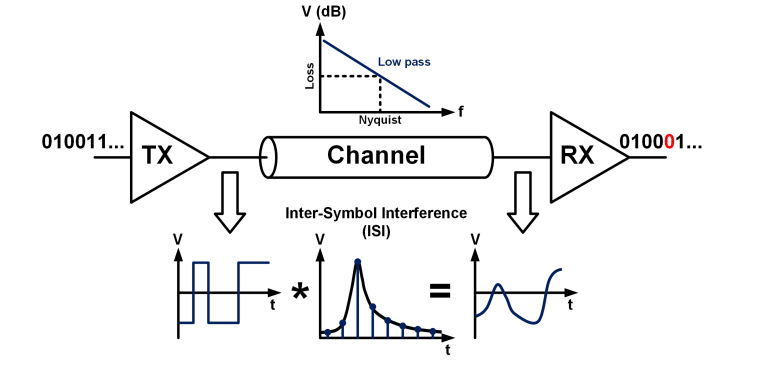
\includegraphics[width=12cm,height=6cm]{fig1.png}
	\caption{Block Diagram of a Simple Communication Channel [4]}
	\label{block_diag}
\end{figure*}

Eye diagrams provide a pictorial way to judge whether a channel/link is healthy. Eye diagrams are generated by overlapping unit intervals (UI) of the signal of interest in the time domain. Figure 1.2 shows examples of open and closed eye diagrams. When channel ISI and noise in the link system is much smaller than the actual data signal, we obtain an open eye diagram (Figure 1.2(a)) in which the eye has a vertical opening, eye height (E.H) and a horizontal opening, eye width (E.W). The dither around the data levels are due to residual ISI and noise. Figure 1.2(b) shows an example of a closed eye diagram. In such a system, ISI and noise overwhelm the transmitted data, therefore making the high and low data levels indistinguishable. For a given PAM scheme, there will be PAM-1 eyes in the eye diagram. \\

\begin{figure*}
	\centering
	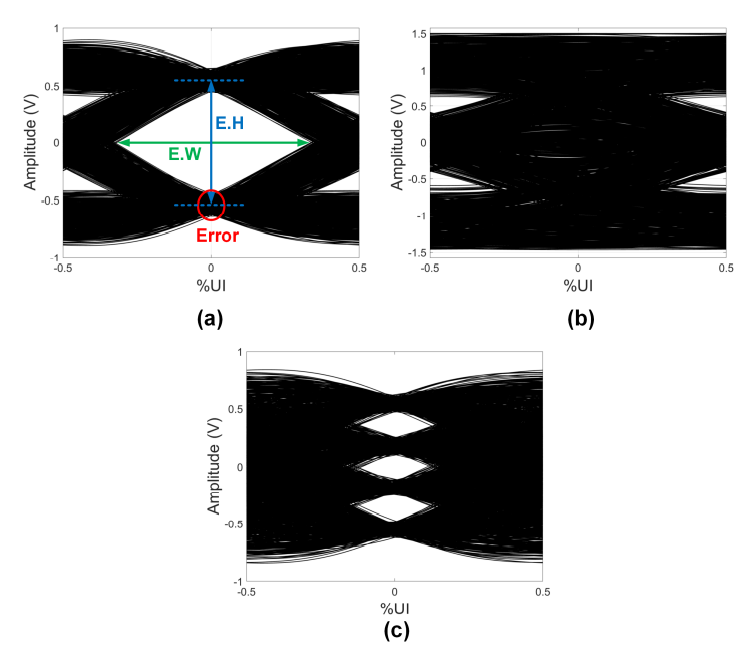
\includegraphics[width=12cm,height=8cm]{fig1_2.png}
	\caption{Examples of (a) an open eye diagram for PAM2, (b) a closed eye diagram
for PAM2 and (c) an open eye diagram for PAM4 [4]}
	\label{PAM_eye}
\end{figure*}

Bit error rate (BER) is the metric that ultimately quantifies a link's performance. As illustrated by the PAM2 example in Figure 1.3, the TX only sends voltages representing either a "0" or "1" in the probability domain. After channel ISI and circuit/environment noise are added, the receiver sees a signal whose probability density function (PDF) is a sum of two Gaussian-like peaks. The area under the curves' crossed-over portions gives the probability of a wrong bit decision, thus BER.\\

\begin{figure*}
	\centering
	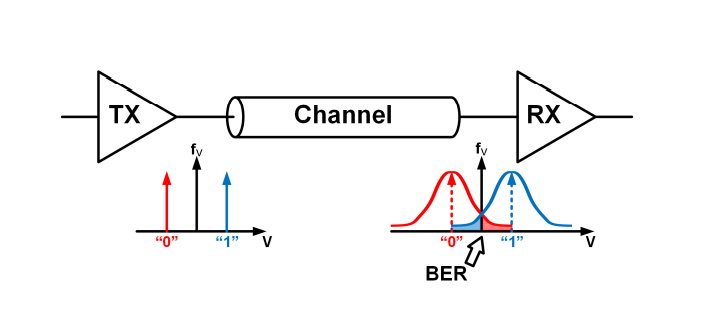
\includegraphics[width=12cm,height=6cm]{fig1_3.png}
	\caption{Bit error rate in wireline links [4]}
	\label{BER_links}
\end{figure*}

In order to compensate for ISI due to channel loss and meet the required BER specifications, different equalization techniques are used in link systems. Figure 1.4 shows conventional mixed-signal equalization blocks on both the TX and RX end [4]. The main cursor in a channel's pulse response is the signal of interest. Any ISI cursors before the main cursor are called pre-cursors. A feed-forward equalizer (FFE), which is typically implemented on the TX side, normally cancels pre-cursors. Any ISI cursors following the main cursor are considered post-cursors, which are often taken care of by the receiver with a continuous-time linear equalizer (CTLE) and decision feedback equalizer (DFE). The CTLE acts as high-pass filter to compensate for the channel's low-pass action. Due to the high-pass nature of CTLEs, any high frequency receiver input noise will be boosted similar to the actual signal. To avoid excessive noise amplification, DFEs pass the noise-less recovered bits through a finite impulse response (FIR) filter that matches the post-cursor portions of the channel to achieve ISI cancellation. The TX FFE can also provide some coarse equalization for post-cursors.

\begin{figure*}
	\centering
	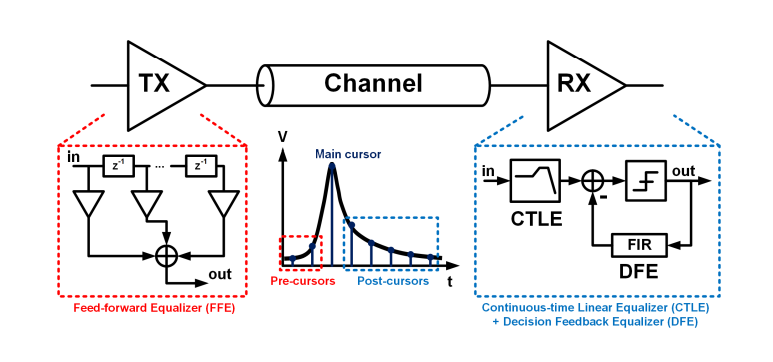
\includegraphics[width=12cm,height=6cm]{fig1_4.png}
	\caption{Equalization in conventional mixed-signal links [4]}
	\label{BER_links}
\end{figure*}


\section{Organization}
\rhead{Organization}
\begin{itemize}
	\item To understand the application space for ADCs	, we first review the 
basic concepts of high-speed link systems in Chapter 2.
	\item In Chapter 3, we look in detail, at the design of a sub-ADC including Sampling switch, StrongARM Latch, SAR Logic and the integration of these elements to form an SAR ADC.
	\item In Chapter 4, we take a look at the preliminary results that we have obtained in the due course of this work thus far.
	\item In Chapter 5, the work to be done in the future will be discussed followed by conclusions.
	\item In Chapter 6, various references have been cited.
\end{itemize}

\newpage

